% !TeX program = xelatex
% !BIB program = biber
\documentclass[portuguese]{textolivre}

% metadata
\journalname{Texto Livre}
\thevolume{18}
%\thenumber{1} % old template
\theyear{2025}
\receiveddate{\DTMdisplaydate{2024}{7}{3}{-1}}
\accepteddate{\DTMdisplaydate{2024}{8}{28}{-1}}
\publisheddate{\today}
\corrauthor{Vinicius Viana Busatto}
\articledoi{10.1590/1983-3652.2025.53269}
%\articleid{NNNN} % if the article ID is not the last 5 numbers of its DOI, provide it using \articleid{} commmand 
% list of available sesscions in the journal: articles, dossier, reports, essays, reviews, interviews, editorial
\articlesessionname{articles}
\runningauthor{Busatto e Pereira}
%\editorname{Leonardo Araújo} % old template
\sectioneditorname{Daniervelin Pereira}
\layouteditorname{João Mesquita}

\newfontfamily\Symbola{Symbola}

\title{A convergência das artes no gênero discursivo \emph{songfic}:
dialogismo, multimodalidade e literatura infanto-juvenil na era
digital}
\othertitle{The convergence of arts in the discursive genre songfic: dialogism,
multimodality, and young adult literature in the digital age}

\author[1]{Vinicius Viana Busatto~\orcid{0000-0001-6935-9108}\thanks{Email: \href{mailto:busattovini@gmail.com}{busattovini@gmail.com}}}
\author[1]{Márcia Helena de Melo Pereira~\orcid{0000-0002-3663-3462}\thanks{Email: \href{mailto:marciahelenad@yahoo.com.br}{marciahelenad@yahoo.com.br}}}

\affil[1]{Universidade Estadual do Sudoeste da Bahia, Programa de Pós-Graduação em Linguística, Departamento de Estudos Linguísticos e Literários, Vitória da Conquista, BA, Brasil}

\addbibresource{article.bib}

\begin{document}
\maketitle
\begin{polyabstract}
\begin{abstract}
Para Bakhtin, os enunciados são únicos e irrepetíveis, portanto
heterogêneos. Por meio das interações sociais, ocorrem transformações
nos gêneros discursivos, que são inúmeros e possuem diferentes
propósitos comunicativos. Dito isso, este artigo investiga um exemplar
de \emph{songfic}, um gênero discursivo contemporâneo em ascensão no
ciberespaço, especialmente, entre o público infanto-juvenil, em que
letras de canções servem de inspiração para ficções de fãs, formando um
elo entre diferentes produtos midiáticos. Para tal, analisamos as
estratégias intertextuais e hipertextuais adotadas nessas narrativas,
bem como as relações dialógicas estabelecidas entre elas e as demais
obras, em um viés bakhtiniano, por meio de um percurso
teórico-metodológico de cunho descritivo-interpretativo, consistindo na
captura de tela e extração de excertos dos exemplares em plataformas
voltadas à publicação das \emph{fics}. Os resultados evidenciam que a
história analisada, \emph{Cry Baby}, de BrookeYoongi, tece referências
às letras das canções por meio de elementos verbo-visuais, estabelecendo
diálogos, além das canções, com videoclipes e outras obras literárias.
Em síntese, esse gênero digital permite explorar leituras e
(ciber)culturas de forma inovadora, graças ao envolvimento ativo dos
fãs-autores na (co)criação de obras artísticas.
  
\keywords{Songfics \sep Gêneros discursivos \sep Dialogismo \sep
Multimodalidade}
\end{abstract}

\begin{english}
\begin{abstract}
According to Bakhtin, utterances are unique and unrepeatable,
and therefore heterogeneous. Through social interactions,
transformations occur in the various discourse genres, which are
numerous and serve different communicative purposes. Therefore, this
article examines an example of songfic, a contemporary discourse genre
on the rise in cyberspace, particularly among the younger audiences, in
which song lyrics serve as inspiration for fan fictions, creating a link
between different media products. To this end, we analyze the
intertextual and hypertextual strategies adopted in these narratives, as
well as the dialogical relations established between them and other
works, from a Bakhtinian perspective, through a
descriptive-interpretative theoretical-methodological approach,
consisting of screenshot capture and the extraction of excerpts from the
examples on specialized platforms. The results show that the analyzed
story, \emph{Cry Baby} by BrookeYoongi, weaves references to the song
lyrics through verbal-visual elements, establishing dialogues not only
with the songs but also with music videos and other literary works. In
summary, this digital genre allows for innovative explorations of
readings and (cyber)cultures, thanks to the active involvement of
fan-authors in the (co-)creation of artistic works.

\keywords{Songfics \sep Discourse genres \sep Dialogism \sep Multimodality}
\end{abstract}
\end{english}
\end{polyabstract}

\section{Introduction}\label{sec-intro}
The educational context is seen as a social ecosystem, exhibiting characteristics of a complex adaptive system, composed of nested systems, such as schools, classrooms, families, and so on. Agents within these systems, such as educators, students, and teachers contribute to the emerging dynamics of their relationships within these systems. An investigation of ecological systems requires lenses that contemplate the possible relationships and dynamics among their agents. The ecological approach is considered a way of thinking and studying organisms in their relationship with the environment. \textcite{vanlier2004} reminds us that this approach is based on systems theory, complexity theory, chaos theory, and cybernetics, recognizing the complexity and interrelationship of the processes that lead to the creation of an environment.


Underpinned by the construct of ecological perspective and coupled with the concept of affordance, this study attempts to better understand how pre-service teachers exercise their agency using mobile digital technologies. The concept of affordance can serve to identify actions arising from these teachers’perceptions. Moreover, we resort to discussions on agency as a complex system in Applied Linguistics \cite{mercer2012, larsen2019} because they can advance our understanding of patterns that emerge from the perception-action relations as these pre-service teachers exercise agency.


The concept of agency is present in discussions of several areas of knowledge and has been on the agenda of Applied Linguistics. Discussions by \textcite{vanlier2004,vanlier2010a,mercer2011,mercer2012,mercer2018,larsen2019}, however, stand out from those of other scholars because they rely on the ecological perspective and complexity theory.


Although the field of Applied Linguistics is not devoid of discussions on these perspectives, the dimensions of pre-service teachers’ exercise of agency mediated by mobile digital technologies have been underexplored, which justifies the development of this study. With that in mind, we seek to identify: 

\begin{enumerate*}[label=\roman*)]
	\item Instances of the agency exercised by pre-service teachers;
	\item Actions mediated by the use of cell phones by these teachers;
	\item Intrapersonal issues (emotions, beliefs, motivation, etc.) that can influence their agency.
\end{enumerate*}


We briefly present the theories and concepts undergirding this study, namely: the ecological approach, complexity theory, mobile learning, and agency.


% !TeX root = main.tex

\section{Fanfiction e cultura participativa: a manifestação do fandom}\label{sec-fanfictionecultura}

No ensaio \emph{Arte e responsabilidade}, \textcite{bakhtin_arte_2003} argumenta que a
\emph{ciência}, a \emph{arte} e a \emph{vida} são os três domínios da
cultura humana e eles só adquirem unidade no indivíduo que os incorpora
em sua própria unidade. Em outras palavras, as diferentes partes desse
todo, a cultura humana, não devem estar ligadas de maneira mecânica ou
externa, como quando ``o homem sai da `agitação do dia a dia' para a
criação como para outro mundo `de inspiração, sons doces e orações'\,''
\cite[p.~33]{bakhtin2011}. Isso resultaria em uma arte vazia e ousada, em
vez de responsiva à vida. \textcite{bakhtin2011} defende que, isto sim, é a
unidade da responsabilidade mútua que garante o elo interno entre os
elementos do indivíduo, ao afirmar que ``Arte e vida não são a mesma
coisa, mas devem se tornar algo singular em mim, na unidade da minha
responsabilidade'' \cite[p.~34]{bakhtin2011}. Consequentemente, essa ideia de
responsividade perpassa grande parte da teoria do autor. De outro modo,
para o pensador russo, viver é agir e a vida é permeada por relações
dialógicas, as quais se voltam tanto para o presente, no aqui e agora,
quanto para o passado/futuro, sempre direcionadas a um \emph{outro} com
o qual \emph{eu} me relaciono. Ao enunciar, tomamos uma posição perante
o próprio mundo, a partir de um lugar social, ideológico e axiológico.

Toda essa interação acarreta tipos de enunciados \emph{relativamente
estáveis}, que circulam em cada campo da comunicação humana e são
denominados ``gêneros do discurso''. Esses gêneros desempenham o papel
de organizar nossa fala e escrita \cite[p.~262]{bakhtin2011}. Eles são
considerados desse modo, porque, embora compartilhem características em
comum, a língua está em constante processo de transformação e os
enunciados não são formas acabadas ou totalmente inflexíveis. Embora
cada enunciação seja inerentemente única, de um ponto de vista
universal, os gêneros são sustentados por três pilares: o \emph{conteúdo
temático}, o \emph{estilo} e a \emph{forma composicional}.

O \emph{conteúdo}, segundo \textcite{bakhtin2010,bakhtin2011}, é um elemento
ético-cognitivo que engloba tanto o assunto evocado no gênero quanto os
aspectos ideológicos, objetivos e posição axiológica subsequentes; é
parte de uma macroestrutura e considera a singularidade do sujeito, sua
vontade e seus conhecimentos, orientando a comunicação discursiva com
abordagem valorativa do objeto e fatores linguísticos, textuais e
discursivos. O \emph{estilo}, por seu turno, abrange escolhas lexicais,
gramaticais e fraseológicas, em um contínuo de mais ou menos
formalidade, refletindo a individualidade do enunciador, mesmo em
gêneros mais regulados. O estilo individual é um epifenômeno do
enunciado, enquanto o estilo do gênero, ligado às práticas da
comunidade, garante sua estabilidade. Por fim, a \emph{forma
composicional} tem a ver com a estrutura geral, a organização textual e
as propriedades particulares do gênero, como a divisão de um artigo em
seções, por exemplo. Esses três pilares estão interconectados no
enunciado: o conteúdo requer uma forma para ser expresso
linguisticamente, o que, por sua vez, implica um estilo, tanto do gênero
quanto individual. Esses elementos estão organicamente integrados no
conjunto do enunciado e são moldados pelo caráter específico de cada
campo de comunicação, conforme orienta \textcite{bakhtin2011}.

Na incessante onda de transformações da \emph{internet} e redes sociais,
os gêneros discursivos também se adaptam e evoluem, assim como o
\emph{e-mail}, descendente da carta tradicional. \textcite{jenkins2009} destaca
três conceitos relevantes para esse fenômeno: a convergência de conteúdo
em múltiplas plataformas, a cultura participativa dos usuários e a
inteligência coletiva dispersa entre as pessoas. Esses elementos
influenciam as \emph{fanfictions} e a cultura midiática em geral.
Autores renomados, como Shakespeare, já faziam uso de ideias alheias em
suas criações antes que surgisse o conceito de propriedade intelectual,
semelhante ao Alonso Fernández de Avellaneda com sua sequência não
oficial de Dom Quixote, em 1614. Logo, a prática de criar obras baseadas
em outras precede a invenção do termo \emph{fanfiction}, no século XX.
Inicialmente, na década de 1930, aparecem os \emph{fanzines}, seguidos
pelas comunidades de fãs que compartilhavam e celebravam seus interesses
comuns. Com a ascensão da internet comercial, os \emph{fandoms}
encontraram um lar, agregando-se e produzindo conteúdo artístico
coletivamente. Em 1998, surge o FanFiction.Net, seguido por outros
fóruns e plataformas. Nessas comunidades \emph{on-line}, os fãs
engajam-se ativamente como criadores, alterando narrativas canônicas e
oferecendo novas perspectivas por meio das \emph{fanfics}.

Retornando às ideias de \textcite{bakhtin2011} sobre gêneros discursivos e
dialogismo, acreditamos que os participantes da interação, nesse
ambiente, são majoritariamente os membros dos \emph{fandoms},
estabelecendo-se um diálogo real e responsivo na confecção de suas
manifestações artísticas. A alternância dos sujeitos, uma das
peculiaridades do enunciado, é marcada por cada publicação ou comentário
nas comunidades, refletindo uma constante relação entre o \emph{eu} e o
\emph{outro}, repleta de retomadas, concordâncias e dissonâncias. Os
fanfiqueiros assumem uma posição axiológica no ato da interação, de modo
que tudo está inserido na arquitetônica da vida real --- da qual fazem
parte os indivíduos que compõem os \emph{fandoms}, considerando um
indivíduo responsável, ativo e responsivo --- e na arquitetônica dos
enunciados. Esses dois aspectos estão interligados porque a vida se
integra à língua por meio de enunciados concretos; e é por meio de
enunciados concretos que a língua adentra a vida, como defende \textcite{bakhtin2011} .

À vista disso, o gênero \emph{fanfiction} está relativamente estável
considerando seus três pilares: o \emph{conteúdo temático}, nesse caso,
está ligado aos aspectos ideológicos dos enunciados, apresentando uma
variedade de temas muito ampla, incapaz de ser mensurada, dada a
quantidade de \emph{fics} publicadas até hoje; o \emph{estilo} é
gerenciado por duas forças importantes: de um lado, o gênero
\emph{fanfiction} e suas características determinadas pelas condições
sócio-históricas que o cercam; de outro, o(s) \emph{ficwriter(s)}, isto
é, o(s) indivíduo(s) por trás daquele novo produto midiático, com suas
marcas pessoais e criativas --- além disso, tendo em vista a
sobreposição do estilo individual, os fanfiqueiros empregam recursos
multissemióticos e construções fraseológicas específicas; por fim, a
\emph{forma composicional} das \emph{fics} é multimodal e adaptável,
dependendo do suporte em que estão inseridas. Elas seguem uma
regularidade na apresentação de informações, como título, pseudônimo,
capa etc. A criatividade e os desejos dos \emph{fandoms} impulsionam as
narrativas, explorando lacunas deixadas nas histórias originais ou
representando comportamentos alternativos ao \emph{mainstream}. Posto
isso, na subseção a seguir, discorremos a respeito de algumas nuances
dos elementos imagéticos que integram as \emph{songfics}.

\subsection{Laços Intertextuais} \label{sub-sec-laços}
  

Constantemente recorremos ao discurso de outras pessoas. De forma geral,
tudo o que dizemos ou interpretamos tem uma origem, que pode ser mais ou
menos visível. Nesse contexto, \textcite{koch2008} retomam
as ideias de Kristeva, autora francesa que cunhou o termo
"intertextualidade" com base em sua interpretação das obras de Bakhtin,
apesar das polêmicas envolvendo essa questão. Para ela, cada texto é um
intertexto, inserido em uma sequência de textos já existentes ou que
ainda serão escritos. Contudo, é importante observar que, em nossa
análise, não consideramos esse conceito como sinônimo de dialogismo.
Isso se deve ao fato de que a intertextualidade se concentra,
majoritariamente, nas relações entre textos; por outro lado, a teoria
bakhtiniana aborda as relações dialógicas de maneira situada, destacando
a natureza responsiva dos enunciados.

Seguindo a mesma lógica, \textcite{koch2008} afirmam que a
Linguística Textual abraça o princípio dialógico de \textcite{bakhtin_marxismo_2009}, reconhecendo que textos estão sempre dialogando com outros e não
podem ser analisados isoladamente. Cada texto interage com seu entorno,
ganhando sentido em relação aos outros. Conforme \textcite{koch2008}, existem duas formas de intertextualidade, quais
sejam: a) estrita, quando há uma presença clara de um texto inserido no
outro; b) ampla, referindo-se a indícios mais sutis ligados ao formato,
estilo ou temas. \apud{barthes_morte_2004}{koch1991}
sustenta que um texto é um mosaico de diferentes textos que lhe dão forma e significado. Portanto, a intertextualidade é semelhante à interdiscursividade, na
medida em que ambos respondem a discursos anteriores, mas o dialogismo é
distinto, pois também está preocupado com as respostas futuras -- cada
enunciado espera por compreensão e resposta ativa, nos termos de \textcite{fiorin_interdiscursividade_2006}. Na prática, neste artigo, usamos interdiscursividade para
descrever relações dialógicas mais amplas, enquanto o conceito de
intertextualidade é utilizado mais especificamente para relações
manifestadas textualmente.

De acordo com \textcite{fiorin_interdiscursividade_2006}, é importante observar que a
intertextualidade sempre implica em uma interdiscursividade, mas o
inverso nem sempre é verdadeiro. Levando isso em conta, podemos analisar
alguns tipos de \emph{intertextualidade estrita}, baseados na obra de
\textcite{genette_palimpsestos:_2010}, conforme apresentado por \textcite{koch2008}: a \emph{citação}, a mais explícita, envolve a inclusão direta de
um trecho de um texto em outro, frequentemente indicado por aspas; o
\emph{parafraseamento} consiste na reformulação de um texto para servir
a diferentes propósitos, públicos ou contextos, resultando em
modificações de sentido; e, por fim, a \emph{alusão estrita} é uma
referência indireta e sutil a um texto, muitas vezes introduzindo
alterações formais e adaptando-o para fins diversos, como humor ou
crítica. Cada uma dessas formas desempenha um papel crucial na
construção do significado.
% !TeX root = main.tex

\section{Songfics: o encontro das artes}\label{sec-songfics}

Consoante a \textcite{bakhtin2011}, os enunciados são únicos, irrepetíveis e
caracterizados pela heterogeneidade, o que leva à diversidade de gêneros
discursivos transformados ao longo do tempo, moldados pela interação
discursiva e variando em diferentes contextos e propósitos
comunicativos. Essas mudanças nas práticas discursivas levam à
transformação dos gêneros, resultando em atualizações em sua composição
e na maneira como são empregados. No tocante às \emph{songfics},
precisamos detalhar o conceito de reelaboração de gênero. \textcite{araujo2009},
fundamentado nas ideias de \textcite{bakhtin_os_1997}, argumenta que a
interação humana é uma das necessidades mais inerentes, resultando na
criação de diversos gêneros em vários campos discursivos aos quais
pertencemos ou com as quais interagimos, como o jurídico, jornalístico,
religioso, acadêmico, entre outros. Conforme esses contextos tornam-se
mais complexos, os próprios gêneros também se tornam mais sofisticados.

Bakhtin utilizou o termo \emph{transmutação} para descrever a
transformação de gêneros complexos, que são empregados em contextos mais
formais, como discursos, artigos e livros, a partir de gêneros
primários, usados em situações cotidianas, como conversas e cartas.
Nesse processo, quando um gênero primário se modifica para se adequar a
um contexto mais formal, muitas vezes, ele assume uma nova natureza,
desvinculando-se da realidade imediata. A transmutação (doravante
\emph{reelaboração}) é um processo constante, o qual os gêneros
complexos estão em constante evolução e adaptação para atender às
necessidades daqueles que os utilizam. No entanto, Bakhtin utilizou esse
conceito especificamente para descrever o fenômeno da formação de
gêneros complexos, que têm origem nos primários. Todavia, hodiernamente,
há casos em que gêneros secundários (complexos) também passam por
transmutação, ou seja, são reelaborados por outros gêneros secundários.

\textcite{araujo2009} ilustra o exemplo do \emph{chat}, que, além de abranger as
conversas cotidianas, também abarcam outros gêneros secundários, como a
aula, a entrevista, a enquete e o material didático, resultando na
formação de uma constelação de gêneros com objetivos variados. Isso se
diferencia das \emph{songfics}, cujo propósito geralmente é mais
específico, qual seja: (re)criar obras artístico-midiáticas, ao passo
que o \emph{chat} pode servir a uma infinidade de funções outras. Neste
caso, há uma negociação do sentido, posto que a canção, ao ser
reelaborada, perde o contato com o seu meio de circulação primário,
tornando-se parte de um novo gênero. Em outras palavras, os gêneros
discursivos têm uma memória, o que significa que eles têm raízes em
gêneros previamente estabelecidos e estão intrinsecamente ligados a um
contexto e a uma comunidade discursiva. No caso das \emph{songfics},
isso está vinculado ao \emph{fandom}.

Nessa perspectiva, a renovação dos gêneros pode assumir, em geral, duas
formas: \emph{transmutação criadora}, quando um gênero inédito, isto é,
com novo propósito comunicativo, surge a partir de outro(s); e
\emph{transmutação inovadora}, quando todo e qualquer gênero, mesmo os
mais estandardizados, comportam transformações, sem que essas o
transformem em um novo gênero. Em essência, as \emph{songfics} (também
conhecidas como \emph{canções-fic}, \emph{ficsongs} ou \emph{fic
músicas}) são narrativas de ficção que incorporam letras de canções, as
quais podem ser intercaladas entre as seções da história ou integradas
ao próprio enredo. A narrativa pode até mostrar personagens ouvindo a
música no rádio e reagindo de acordo ou apresentar momentos da história
nos quais a música desempenha um papel relevante. Além disso, as
\emph{songfics} podem incluir recursos multimodais, como
\emph{hiperlinks}, GIFs, imagens e vídeos, juntamente às estratégias
intertextuais discutidas anteriormente.

Em relação às \emph{fanfictions}, a principal diferença não está no
suporte, mas na maneira como as \emph{songfics} incorporam e utilizam
letras de músicas como parte integrante da narrativa. A diversidade de
abordagens e manipulações nas histórias é vasta e depende dos interesses
e desejos dos \emph{fandoms} que estão espalhados pela internet. Cada um
deles desenvolve suas próprias interpretações criativas e variações das
narrativas, criando uma rede rica e multifacetada de conteúdo dentro
desse universo, de modo que cada sujeito apresenta seu assento
valorativo diante do tema a partir de sua própria dimensão ideológica.
Nessa direção, \textcite{jenkins_textual_1992} aponta dez maneiras pelas quais esse
processo é realizado:

\begin{enumerate}
\def\labelenumi{\arabic{enumi})}
\item
  Recontextualização, que consiste no preenchimento de lacunas na
  história original, explorando as ações não descritas ou mesmo a
  psicologia das personagens;
\item
  Expansão da Linha Temporal, que se refere à narração de eventos não
  mencionados no passado ou futuro da narrativa, sem contradizer o
  cânone;
\item
  Refocalização, que narra a história a partir da perspectiva de
  personagens secundárias ou marginalizadas;
\item
  Realinhamento Moral, a qual compreende transformar vilões em
  protagonistas e explorar suas perspectivas, razões etc.;
\item
  Troca de Gênero, que enfatiza elementos como o romance em histórias
  que não o destacam;
\item
  Crossovers, a prática de unir personagens e cenários de diferentes
  histórias;
\item
  Deslocamento de Personagem, quando personagens são retirados de seus
  contextos originais e então inseridos em situações diferentes;
\item
  Personalização, que se refere à transposição de personagens para novos
  ambientes, a ponto de se trocar características físicas, nome, idade
  etc.;
\item
  Intensificação Emocional, de modo que momentos de crise emocional são
  focalizados nas fics, como um término ou situação traumática, por
  exemplo;
\item
  Erotização, ao serem explorados aspectos eróticos da narrativa, sem
  restrições editoriais e, neste caso, restrito ao público maior de
  idade.
\end{enumerate}

Independentemente das diferentes formas de criação literária, o conceito
de dialogismo de \textcite{bakhtin2011} está sempre presente. Esse fenômeno
reflete a natureza inerente da interação que rege nossos contatos
sociais, sendo fundamental para a capacidade de formular e expressar
qualquer discurso ou enunciado. É o diálogo constante entre vozes,
pontos de vista e influências que enriquece e molda a complexidade das
criações literárias, como as \emph{fics}, e, de fato, todas as formas de
comunicação humana. No diagrama abaixo, apresentamos um breve fluxo que
descreve a formação das \emph{songfics}:

\begin{figure}[htbp]
    \centering
    \begin{minipage}{.75\textwidth}
    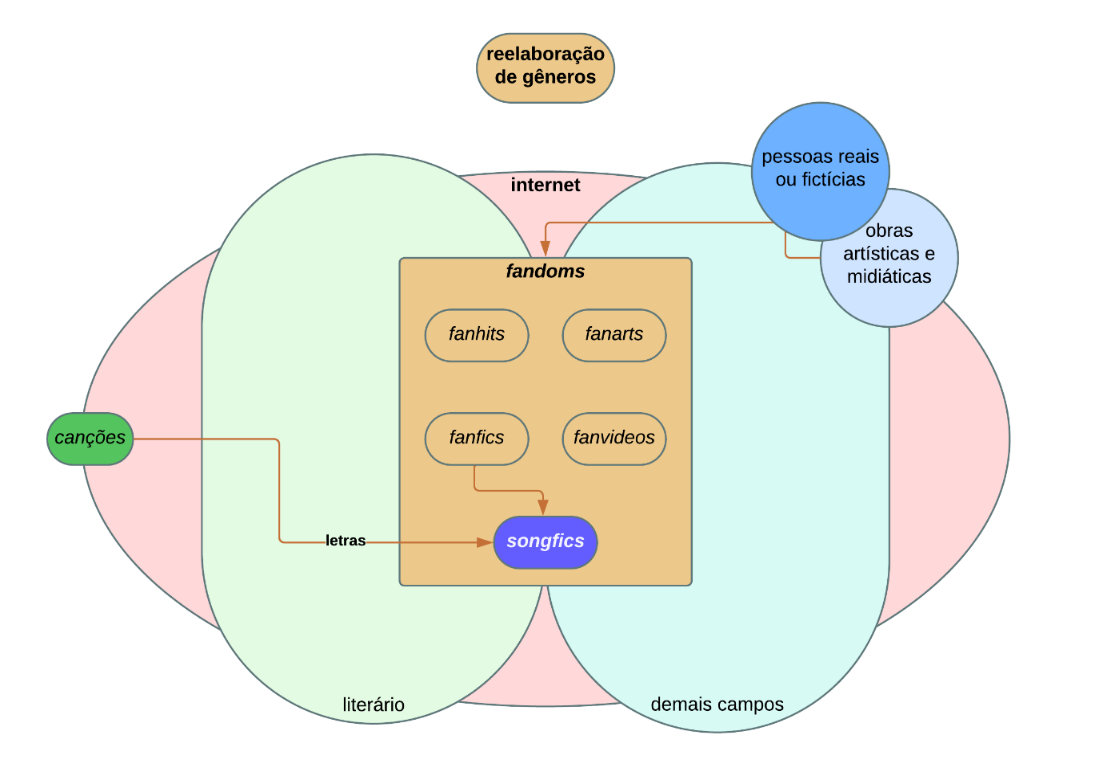
\includegraphics[width=\textwidth]{fig01.png}
    \caption{O surgimento das songfics.}
    \label{fig-01}
    \source{Elaboração própria.}
    \end{minipage}
\end{figure}

É importante notar que o ambiente predominante em que essas criações
circulam é a internet (em rosa), que serve como o local de encontro e de
interação para diversos \emph{fandoms} (comunidades de fãs) existentes.
Esses grupos de fãs produzem uma variedade de conteúdos com base em
pessoas reais ou fictícias (em azul) e em obras artísticas e midiáticas
(azul-claro), que constituem o principal \emph{input} para a criação de
\emph{fanhits}, \emph{fanarts}, \emph{fanvideos}, \emph{fanfics} e
outros tipos de produções. Estas últimas, além de serem influenciadas
por esses elementos, também são alimentadas pelas letras de canções (em
verde), que servem de inspiração para a criação das \emph{songfics} (em
roxo), por meio de um processo de \emph{reelaboração}. Esse diagrama
ilustra como as \emph{songfics} se encaixam em um contexto mais amplo de
criação de conteúdo dentro dos \emph{fandoms}, destacando a interconexão
entre diferentes formas de expressão criativa. De modo mais específico,
vejamos, na \Cref{fig-02}, o fluxo desse gênero:


\begin{figure}[htbp]
    \centering
    \begin{minipage}{.5\textwidth}
    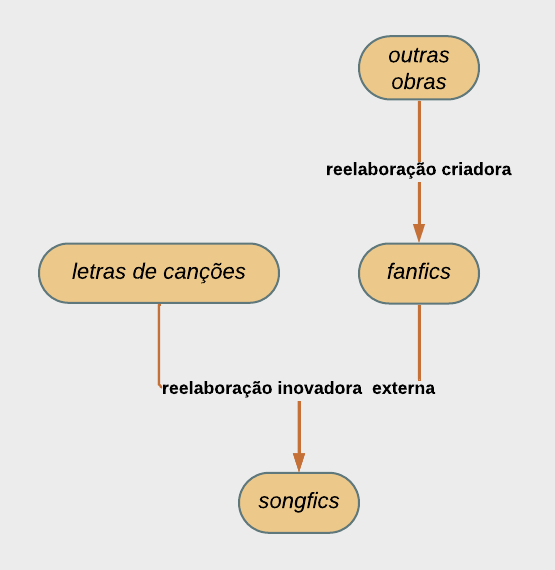
\includegraphics[width=\textwidth]{fig02.png}
    \caption{Reelaboração.}
    \label{fig-02}
    \source{Elaborado com base em \textcite{araujo2009}.}
    \end{minipage}
\end{figure}

De forma ampla, as \emph{fanfictions} são escritas com base em obras
pré-existentes, como filmes, séries, jogos etc., com o objetivo de
expandir, recriar ou modificar o universo ficcional originário,
resultando na criação de uma literatura não oficial. Esse processo pode
ser considerado como uma forma de \emph{reelaboração criativa}, uma vez
que um gênero é gerado a partir de outro. Nesse contexto, o propósito e
a função são alterados, já que as \emph{fanfics} lançam uma nova
perspectiva sobre a obra e atendem a um público específico, os
\emph{fandoms}, que empregam diversas estratégias de reinterpretação
para personalizar suas criações. Nessa cultura participativa, como
descrita por \textcite{jenkins2009}, os consumidores (\emph{ficwriters}, no caso
das \emph{fanfics}) interagem ativamente com os produtores das obras
originais, seguindo um novo conjunto de regras e níveis de poder. Os
meios de comunicação contemporâneos democratizaram esse processo. No
entanto, no contexto das \emph{songfics}, os fanfiqueiros decidem
incorporar outro elemento às suas histórias: as letras de canções. Isso
leva à \emph{reelaboração inovadora externa}, uma vez que um gênero
(\emph{fanfiction}) passa a incluir elementos de outro gênero (letras de
músicas). Isso ocorre sem comprometer a função original das
\emph{fanfics}, que é recriar outras obras artísticas. O que acontece,
na verdade, é a introdução de um novo elemento capaz de transformar
internamente um gênero já flexível por natureza.

Com recursos intergenéricos, intertextuais e multimodais, os
\emph{ficwriters} têm à disposição uma nova forma de expressão
artística: a \emph{songfic}. Este gênero permite que três vozes ressoem:
a voz da referência primária (a obra original, a pessoa etc.), a voz da
canção e, não menos importante, a voz do próprio autor que a escreve. O
diálogo entre essas forças coloca a \emph{songfic} em constante fluxo
dialógico da língua, enriquecendo a diversidade das criações literárias.
Com o público infanto-juvenil, portanto, constrói-se um leque de
possibilidades deveras abrangente, em um campo ainda preterido pela
academia e críticos mais tradicionais. Na vida escolar, a incorporação
de recursos e tecnologias multimidiáticas tem ocorrido gradualmente,
porém em um ritmo menos acelerado em comparação ao cotidiano fora das
instituições de ensino, de acordo com \textcite{damiani2016}. Com isso em mente,
a seguir, vejamos a análise de um exemplar de \emph{songfic} que dialoga
com múltiplas linguagens e mídias.
\section{Metodologia}\label{sec-metodologia}

Não foi necessária uma análise ética prévia por parte dos conselhos de
projetos adequados para a investigação, uma vez que os participantes não
foram identificados. Por não haver conflito de interesses, a Texto Livre
não terá quaisquer consequências, inclusive assistência integral e
eventual, ressarcimento de qualquer dano resultante a qualquer dos
participantes da pesquisa, conforme a Resolução nº 510, de 7 de abril de
2016, do Conselho Nacional de Saúde do Brasil.

A metodologia é a explicação minuciosa, detalhada, rigorosa e exata de
toda a ação desenvolvida no método de trabalho da pesquisa \cite{lakatos2003}. A pesquisa é um estudo de caso, que teve o aluno como
objeto de estudo. \textcite[p. 32]{yin2005} argumenta que o estudo de caso visa a \enquote{conhecer em profundidade o como e o porquê de uma determinada
	situação que se supõe ser única em muitos aspectos, procurando descobrir
	o que há nela de mais essencial e característico}. O estudo de caso é
caracterizado pelo estudo profundo e exaustivo de um ou poucos objetos,
de maneira a permitir o seu conhecimento amplo e detalhado. O caso
experimental caracteriza-se por determinar um objeto de estudo,
selecionar as variáveis que seriam capazes de influenciá-lo, definir as
formas de controle e de observação dos efeitos que a variável produz no
objeto \cite{gil2002}. A coleta dos dados foi realizada em uma escola
secundária do sul de Moçambique. Fizeram parte da amostra 50 alunos do
ensino secundário, selecionados de forma aleatória, dos quais 25
participaram do estudo das PO e aplicação do Q3DM. Os restantes 25
estiveram envolvidos no estudo das SCs e aplicação do GeoGebra. Em ambos
os estudos, todos os alunos experimentaram as aplicações (Q3DM ou
GeoGebra). A pesquisa apresenta um estudo de caso interpretativo, o qual
desenvolve categorias conceituais indutivamente para examinar os
pressupostos iniciais, as intenções e significados das ações e
expressões dos alunos \cite{amado2017}. A compreensão interpretativa é
sustentada a partir do relato pormenorizado da interação dos sujeitos em
seu meio natural \cite{coulon1995}. A visão interpretativa descreveu as
ações dos alunos em ambiente de sala de aula e os significados das ações
no processo de toda a pesquisa \cite{coutinho2011}.

Foi possível, pois, observar e interpretar tudo o que ocorreu, tornando
viável a análise das relações causa-efeito. Foi possível , também,
qualificar as ações dos alunos em todo o processo de aprendizagem, por
meio das interpretações dos significados de seus comportamentos durante
a mediação da aula e as respostas do questionário de satisfação. Além
disso, os dados foram coletados por meio das técnicas de observação do
participante, com tomada de notas e de registro fotográfico, assim como
dos instrumentos de coleta de dados aplicados, como os questionários de
satisfação.

\subsection{Realização das aulas}\label{sub-sec-Realização das aulas}

As aulas consistiram na apresentação de dois temas, PO e SCs, de forma
separada. Para os alunos da 9ª classe, o tema de pesquisa foi PO, e foi
utilizado o Q3DM. A professora primeiramente apresentou o tema,
explicando o que eram POs, dizendo que eram figuras geométricas sobre um
plano que poderiam ser comparadas à sombra do mesmo objeto no horário em
que o sol estaria no ponto mais alto no dia. Depois, demonstrou as
vistas ortogonais do sólido. (Ver \Cref{fig-03}).

\begin{figure}[htpb]
\centering
\begin{minipage}{.5\textwidth}
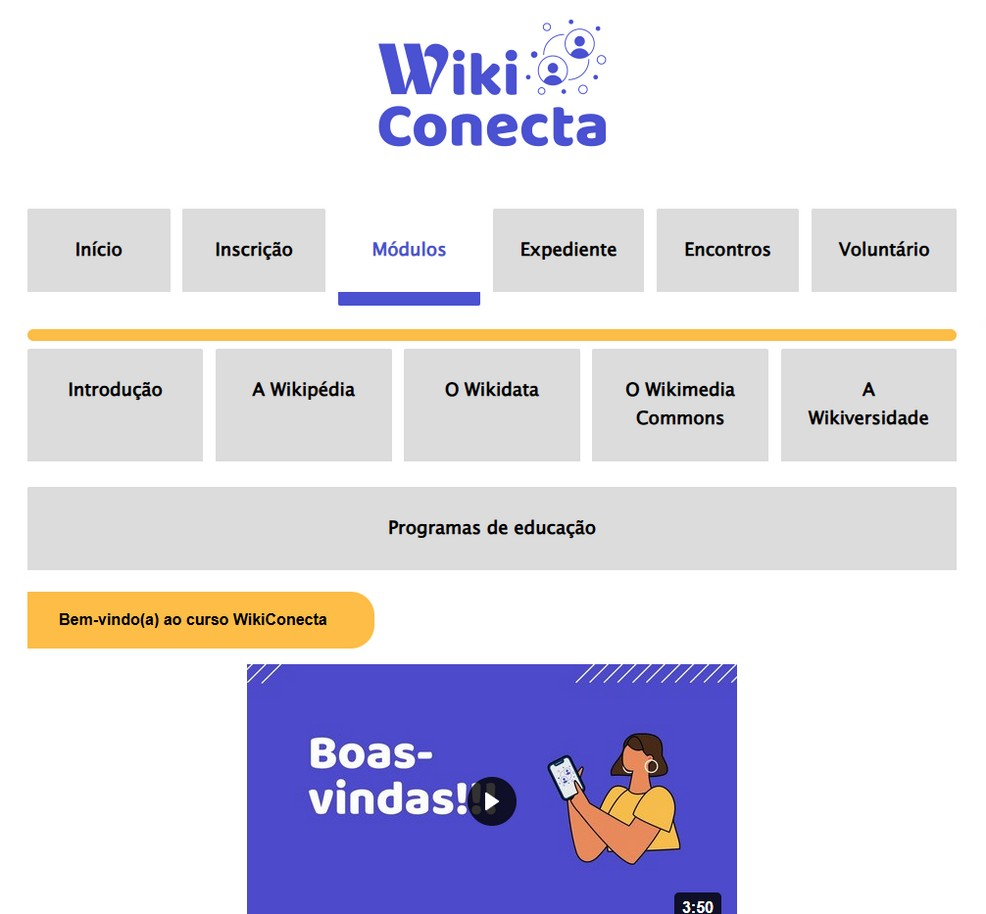
\includegraphics[width=\textwidth]{figures/figure03.jpg}
\caption{Vistas ortogonais e ortográficas: vista frontal; vista superior; e vista lateral esquerda.}
\label{fig-03}
\source{\url{http://turmag1215vialonga.blogspot.com/2014/10/projecoes-ortogonais.html}.}
\end{minipage}
\end{figure}

Posteriormente a professora apresentou a aplicabilidade das POs, dizendo
que eram destinadas à planificação de vários objetos. Com o auxílio das
simulações computacionais, construiu os sólidos geométricos e demonstrou
suas vistas ortogonais, apresentando os procedimentos para a manipulação
do Q3DM. (Ver \Cref{fig-04})

\begin{figure}[htpb]
\centering
\begin{minipage}{.5\textwidth}
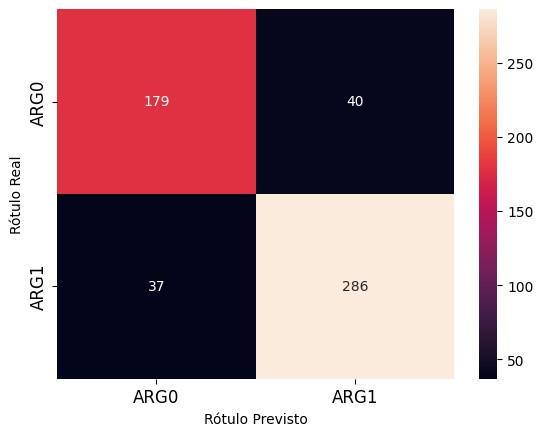
\includegraphics[width=\textwidth]{figures/figure04.jpg}
\caption{Manipulação no Q3DM.}
\label{fig-04}
\source{Elaboração própria.}	
\end{minipage}
\end{figure}


A manipulação no Q3DM é feita por meio de cubos chamados Qubes, que
facilitam a criação e a montagem de objetos em três dimensões,
utilizando elementos digitais que podem ser inseridos, removidos,
deslocados, ampliados, inclinados, moldados geometricamente, girados e
coloridos.

Para os alunos da 12ª classe, o tema de pesquisa foi SCs e foi utilizado
o GeoGebra. A professora iniciou com a apresentação do tema SCs de
cilindro, explicando que a seção cilíndrica é uma figura resultante de
um plano secante no cilindro. A professora acrescentou que existem duas
situações distintas: quando o plano secante é paralelo ao eixo central
do cilindro; e quando o plano secante não é paralelo ao eixo central do
cilindro (ver as figuras \Cref{fig-05} e \Cref{fig-06}).

\begin{figure}[htpb]
\centering
\begin{minipage}{.25\textwidth}
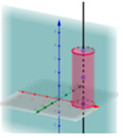
\includegraphics[width=\textwidth]{figures/figure05.jpg}
\caption{Secção paralela ao eixo central do cilindro.}
\label{fig-05}
\source{Elaboração própria.}
\end{minipage}
\end{figure}

\begin{figure}[htpb]
\centering
\begin{minipage}{.5\textwidth}
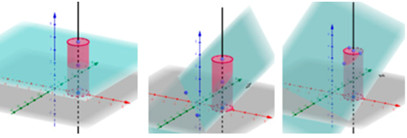
\includegraphics[width=\textwidth]{figures/figure06.jpg}
\caption{Secção não paralela ao eixo central do cilindro.}
\label{fig-06}
\source{Elaboração própria.}
\end{minipage}
\end{figure}

A professora, primeiramente, apresentou os diferentes posicionamentos
dos planos em relação ao eixo central do cilindro. Em seguida, com o
auxílio da tecnologia, apresentou à turma o software de geometria
dinâmica GeoGebra, indicando as funcionalidades de suas ferramentas e
como construir do ponto até o plano secante, com a ajuda dos
procedimentos para a sua manipulação no GeoGebra. Os alunos simularam as
SCs com o plano de nível; eles apresentaram-se atentos e motivados em
aprender a resolver o exercício no GeoGebra, particularmente para os
rapazes, os quais procuravam descobrir como construir diferentes sólidos
geométricos e como simular as VOs (vistas ortogonais).

\subsection{Realização do questionário}\label{sub-sec-Realização do questionário}

O questionário de satisfação aplicado teve como objetivo compreender se
o Q3DM e o GeoGebra facilitaram a aprendizagem das POs e SCs, e se o
\textit{smartphone} foi fácil de manipular. Ambos os questionários foram
preenchidos em 10 minutos. As questões visavam a coletar, nos dois
estudos, várias opiniões, incluindo: (1) se os aplicativos tecnológicos
facilitaram as representações 3D; (2) qual é a opinião deles sobre os
benefícios de usar os aplicativos ou se seria melhor resolver de forma
tradicional; (3) se os aplicativos são fáceis e intuitivos de usar; (4)
quais foram os aspectos positivos e negativos da aula; e, (5) como eles
classificariam a aprendizagem com o auxílio dos aplicativos.

\section{Análise}\label{sec-análise}

Nesta seção, realizaremos a análise dos 21 artigos selecionados para a
revisão sistemática de literatura sobre o conceito de literacia
algorítmica (LA). Todos os artigos analisados estão detalhados em tabela
no (\Cref{anexo-1}), que inclui o nome dos/das autores/as, ano da
publicação, título do artigo, tipo e local de publicação. Inicialmente,
apresentaremos uma análise dos metadados das publicações, entre eles o
ano de publicação, autores, periódicos ou eventos em que foram
apresentadas, junto a outros detalhes relevantes. Em seguida, realizamos
efetivamente a análise do \emph{corpus}, considerando as questões que
dirigem nossa investigação.

\subsection{Perspectivas iniciais a partir dos metadados}\label{sub-sec-perspectivasiniciais}

Ao analisar a lista de publicações, observamos que os dados abrangem um
período de quatro anos, de 2019 a 2022 (\Cref{image-02}). Notadamente, a
maioria das publicações se concentra nos anos de 2021 e 2022, quando
encontramos, respectivamente, 6 e 10 publicações. Essa concentração do
debate sobre o conceito de LA nos últimos quatro anos, assim como a
tendência ascendente do número de publicações sobre o tema, pode indicar
o aumento do reconhecimento da importância da compreensão dos algoritmos
e seus papéis na vida social contemporânea, bem como o avanço das
discussões em torno da LA.

\begin{figure}[!h]
\centering
\begin{minipage}{0.85\linewidth}
\caption{Número de publicações por ano.}
\label{image-02}
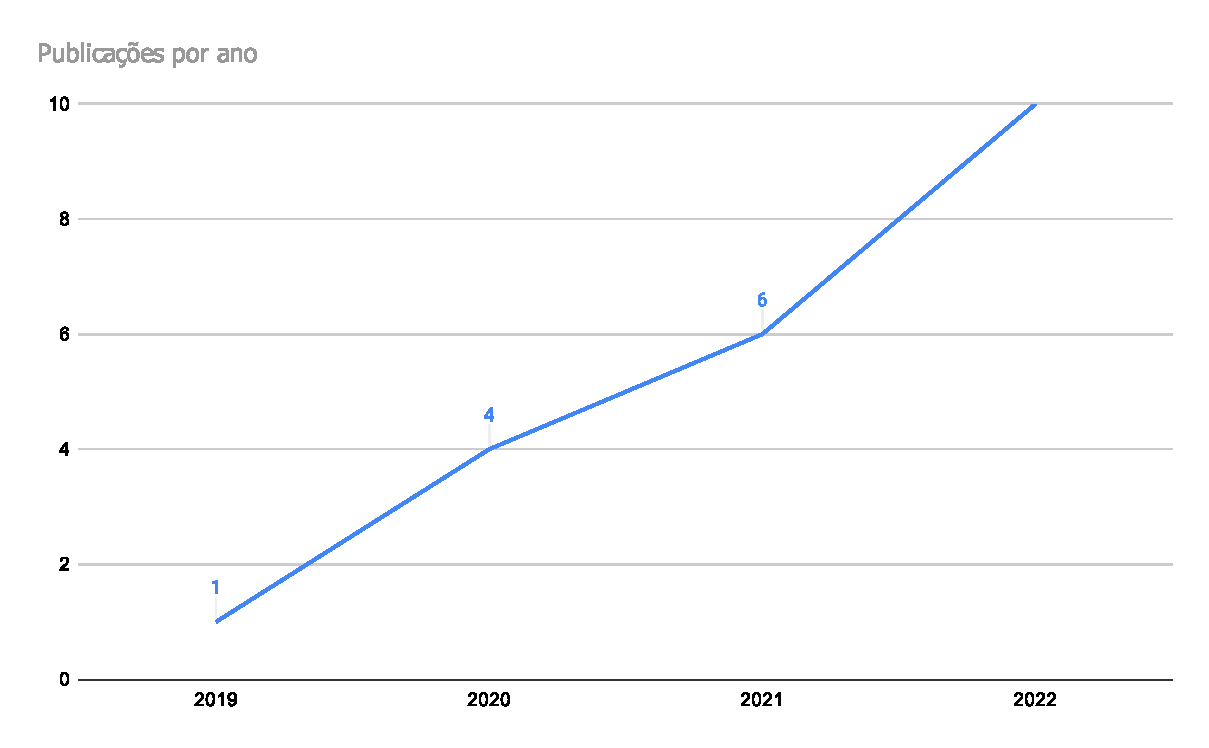
\includegraphics[width=\linewidth]{image2.pdf}
\source{Elaboração própria.}
\end{minipage}
\end{figure}

Em relação à origem das publicações, é possível observar uma diversidade
de formatos, abrangendo artigos em periódicos (15), capítulos de livros
(2) e artigos em anais de eventos acadêmicos (4). Conforme se vê na
tabela do \Cref{anexo-1}, apenas dois periódicos contêm mais de um artigo sobre
o tema (\emph{AI and Society} e \emph{Computers and Composition}).
Nota-se que os estudos encontrados abarcam uma ampla gama de áreas:
comunicação, computação, psicologia, ciência da informação, educação,
além de outras disciplinas relacionadas ao debate sobre tecnologias da
informação e comunicação (como a Interação Humano-Computador). Esse
aspecto pode indicar o interesse multidisciplinar no tema e a relevância
da noção de LA em diversos contextos acadêmicos.

Nessa etapa da análise, também foi percebida a ausência de textos em
português e o baixo número de publicações em espanhol entre os 21
artigos selecionados para a revisão sistemática sobre LA. Essa
observação pode indicar um cenário de escassez de investigações sobre o
tema no contexto latino e ibero-americano.

Com essas informações como base, a próxima etapa da nossa análise
aprofunda o estudo dessas publicações, considerando as questões
orientadoras da investigação sobre propostas conceituais, técnicas
pedagógicas, aplicações práticas e dificuldades relacionadas à LA.

\subsection{Explorando os fundamentos da literacia algorítmica: modelos
conceituais, distinções e aplicações multidisciplinares}\label{sub-sec-explorandoosfundamentos}

A análise dos artigos que abordam a LA revela um cenário diversificado e
complexo, no qual não se observa uma unidade conceitual. Inicialmente,
nota-se que o debate em torno da LA tem propostas que derivam de
abordagens de literacia preexistentes e mais consolidadas, como a
literacia informacional, a literacia para o ambiente digital e a
literacia para os dados \cite{Lloyd2019}. Essas abordagens enfatizam o
processo de criação de consciência individual sobre como a informação é
produzida, classificada e distribuída em diferentes ambientes \cite{Bakke2020}. Nestes estudos, a LA emerge como resposta aos efeitos da
introdução da agência algorítmica, uma série de competências mais
específicas no cenário de uma vida dataficada \cite{Kampa2021}.
Neste contexto, os apelos por literacias são frequentemente uma resposta
a novas tecnologias que criam novas estruturas de poder \cite{Devito2021}.

Para \textcite[p.~3]{Ridley2021}, LA é um dos desdobramentos das
variadas literacias do mundo digitalizado: ``Embora cada uma delas tenha
seu próprio domínio e foco, elas compartilham ideias comuns e geralmente
são simbióticas entre si'' \textcite[p.~3]{Ridley2021}. De modo
similar, \textcite[p.~30]{Devito2021} sustenta que a LA não deve ser observada
isoladamente, mas sim como ``um componente de uma literacia de
plataforma mais ampla que abrange todas as literacias mencionadas
anteriormente''. Para \cite{Lloyd2019}, o que difere a LA de propostas de
literacias mais gerais é que ela necessita de um exame aprofundado da
cultura de desenvolvimento desses sistemas, movimento que vai ao
encontro de propostas de investigação como a de \textcite{Seaver2017}. ``De
acordo com esta perspectiva, a construção de um algoritmo é uma prática
que está inserida dentro de outras práticas e é influenciada por visões
específicas do mundo'' \cite[p.~1483]{Lloyd2019}.

Nesse contexto, a especificidade da LA em relação a outras abordagens
pedagógicas do digital reside na necessidade de um exame crítico de
propriedades características da agência algorítmica, a partir de noções
como performatividade, opacidade, diversidade, confiança, viés e justiça
social \cite{Lloyd2019}. Complementarmente, \textcite{Devito2021} indica que
qualquer proposta de LA deve lidar com a natureza movediça dos sistemas
algorítmicos em constante transformação, incorporando nas construções
pedagógicas essa flexibilidade e capacidade de atualização. Para a
autora, isso faz com que seja fundamental reconhecer que ``os sujeitos
já estão imersos no ambiente em questão, tornando a LA um exercício
principalmente de formalizar e corrigir o conhecimento encontrado no
mundo, em vez de introduzir conhecimentos puramente novos'' \cite[p.~3–4]{Devito2021}.

Nos estudos analisados, um dos objetivos centrais para a LA é o
desenvolvimento de consciência sobre a agência dos sistemas algorítmicos
nas diferentes interações com os sujeitos \cite{Bakke2020}, seja na busca
por informações e conteúdos \cite{Kampa2021}, na interação com
sistemas de interação automatizados \cite{Shin2022} ou na relação com a
personalização algorítmica \cite{Devito2021,Lv2022,Bell2023}. Trata-se, segundo \textcite{Ridley2021},
de uma maneira de reconhecer e dar consciência sobre as formas de poder
deste padrão tecnológico e, ao mesmo tempo, enfatizar os empoderamentos
possíveis aos sujeitos diante dessas estruturas. Nesta abordagem, a LA
pode ser definida como a capacidade de estar ciente tanto da presença
quanto dos desdobramentos de sistemas conduzidos algoritmicamente e,
assim, cristalizar essa compreensão em um uso estratégico desses
sistemas para que os sujeitos integrantes desse processo possam alcançar
objetivos individuais ou coletivos \cite{Devito2021}. Dessarte, LA deve ser
entendida como mais do que instruções para um uso mais eficiente de
sistemas algorítmicos. Ela é uma prática ideológica de produção de
sentido e de subjetivações dissonantes ao que a performatividade desses
sistemas permite \cite{Ridley2021}.

No próximo segmento deste item da análise, serão exploradas duas
dimensões constituintes dos debates que emergem dos artigos examinados.
Primeiramente, será discutido o significado da noção de empoderamento
crítico. Depois, será abordado o espectro dos diferentes níveis de
consciência dos sujeitos em relação aos sistemas algorítmicos. Ambos os
debates são centrais para as propostas conceituais de LA analisadas.

\subsection{Empoderamento crítico: caminhos da agência diante de
sistemas algorítmicos}\label{sub-sec-empoderamentocritico}

Poder e controle são duas noções centrais no debate estabelecido pela
literatura crítica sobre algoritmos. \textcite{Magalhaes2018} sustenta que parte
da literatura, que chama de \emph{paradigma do dano}, considera o poder
dos algoritmos como resultado e também como impulsionador de uma
disparidade original entre os sujeitos (que têm suas vidas afetadas pela
análise de dados digitais sem estarem cientes disso) e os operadores das
plataformas (que deliberada e estrategicamente controlam a coleta e a
análise desses dados). Conforme indica \textcite{Rieder2018}, essas abordagens
estão orientadas, muitas vezes, a apenas denunciar os efeitos políticos
e sociais dos sistemas algorítmicos, negligenciando a análise de como
essas infraestruturas se articulam material e discursivamente para
produzir os efeitos de poder.

Na análise dos artigos da amostra, nos parece claro que poder e controle
são questões para as quais as investigações analisadas buscam oferecer
algum tipo de resposta ou abordagem crítica. Neles, a LA tende a ser
posicionada enquanto conhecimento pedagógico para o desenvolvimento de
consciência crítica e, consequentemente, ampliação da capacidade de
agência dos sujeitos. É neste contexto que emerge a noção de
\emph{empoderamento crítico} como resultado esperado da LA. Nas
propostas conceituais analisadas há ênfase em um empoderamento
individual a partir da capacidade de observar criticamente os modos de
funcionamento desses sistemas \cite{Bakke2020,Konig2022}.

\textcite{Konig2022}, por exemplo, sustenta que a LA pode formar sujeitos com
uma postura reflexiva em relação a sistemas algorítmicos, permitindo que
compreendam que, a cada sugestão ou resultado gerado por esses sistemas,
há trações de objetivos, interesses e suposições que não necessariamente
estão claros. De modo similar, \textcite[p.~1483]{Lloyd2019} entende que os
processos de reflexão são centrais nas literacias, por isso podem
colaborar para gerar atenção sobre como ``os algoritmos são expressos e
operacionalizados (por meio de nossas ações e interações com interfaces
e programas), juntamente com as condições, suposições e vieses que são
inerentes à sua produção e operacionalização.'' \textcite[p.~177]{Sued2022}
indica que a consciência crítica e o conhecimento desenvolvidos a partir
da LA podem garantir aos sujeitos ``um maior agenciamento e liberdade de
ação''.

Porém, adverte \textcite{Konig2022}, o \emph{empoderamento crítico} como
resultado da LA revela-se limitado por duas razões. Primeiramente, o
efeito de uma compreensão crítica dos algoritmos é naturalmente
restrito, já que não há garantias de que as pessoas poderão incorporar
esses conhecimentos e atitudes para exercer controle sobre as operações
de um sistema algorítmico. As configurações, interfaces e regras desses
sistemas, muitas vezes, atuam para limitar as possibilidades de escolha
individual. Mesmo que seja possível conceder aos usuários mais controle
por meio de influência individual sobre a configuração e o comportamento
do sistema, permanece um segundo obstáculo: a produção de uma postura
mais ativa e engajada desses sujeitos no processo de definição dos seus
objetivos, interesses e valores dentro desses sistemas.

Portanto, no debate sobre LA, a capacidade de desenvolver uma
consciência crítica em relação a sistemas algoritmos é vista como
caminho para ampliar a agência dos sujeitos, uma resposta crítica. Nesse
sentido, em conformidade com a abordagem de \textcite{Siles2024}, consideramos
que o debate sobre LA está imbricado com a noção de agência. Ao olhar o
que as pessoas fazem com os algoritmos, \textcite{Siles2024} propõe uma
abordagem de agência mais fluida, que deriva da bricolagem entre
discussões dos Estudos Culturais e dos Estudos de Ciência e Tecnologia.
Nessa proposta, a relação com algoritmos passa a ser vista menos como
polos opostos sólidos ou estados definitivos e mais como relações de
convergência, instabilidade, coexistência, fricção e mudança. Às vezes
os usuários seguem as sugestões dos algoritmos, outras vezes resistem a
elas. Muitas vezes, têm as duas posturas nas mesmas ações. Passa-se a
considerar que a agência é um processo relacional que se dá no espaço
intermediário da relação entre sujeitos e algoritmos \cite{Siles2024}.

No próximo item, são discutidas reflexões sobre os diferentes níveis de
consciência sobre o funcionamento de sistemas algorítmicos, um ponto de
destaque na literatura acerca do tema.

\subsection{Níveis de consciência e percepção sobre algoritmos}\label{sub-sec-niveisdeconscienciaepercepção}

A consciência sobre a existência e funcionamento de algoritmos é um tema
recorrente nas discussões sobre plataformas digitais. As pesquisas
iniciais, realizadas na metade da década anterior, indicaram um baixo
nível de consciência sobre a existência e o funcionamento dos algoritmos
\cite{Eslami2015}. \textcite{Bucher2019}, por exemplo, investigou o
modo como as pessoas tomam consciência sobre a agência algorítmica,
sugerindo que os imaginários sobre o funcionamento desses sistemas podem
condicionar a forma como esses indivíduos desenvolvem suas práticas em
uma determinada plataforma.

Nos debates observados em nosso estudo, a percepção dos sujeitos sobre
algoritmos é posicionada como fator central na literacia algorítmica
(LA), a partir da premissa de que as formas de compreensão sobre esses
sistemas podem moldar significativamente as práticas e interações dos
sujeitos com os ambientes digitais. Nos estudos observados na amostra
analisada, notam-se diferentes abordagens que dialogam com esta questão.
\textcite{Bell2023} apontam que a consciência sobre o
funcionamento de sistemas algorítmicos pode variar dramaticamente em um
grupo semelhante. No estudo, indica-se que a percepção sobre sistemas
algorítmicos pode variar entre plataformas e costuma ser mais
verbalizada quando se fala de serviços nos quais sistemas de
personalização são mais proeminentes no uso, como o TikTok \cite{Bell2023}. Segundo as autoras, essa percepção inclusive pode
depender da maneira como o tema é colocado aos sujeitos (por exemplo, a
partir da variação dos termos escolhidos, como algoritmo ou
personalização). Já a pesquisa de \textcite{Lv2022} correlaciona
essa consciência com a intenção dos adolescentes de resistir aos
algoritmos em plataformas \textit{on-line}. Para as autoras, os diferentes níveis
de conscientização e conhecimento sobre algoritmos estão relacionados à
disposição de os adolescentes buscarem formas de lidar ou evitar esses
sistemas \cite{Lv2022}. O estudo de \cite[p.~352]{Parnell2022}, que analisa as consultas a buscadores \textit{on-line}, apresenta
achados empíricos que indicam que ``uma maior literacia algorítmica tem
um efeito positivo nas habilidades autorrelatadas no uso de sistemas de
busca e no uso mais frequente da Internet''.

É possível perceber nesses estudos um esforço para a criação de
parâmetros que tornem possível mensurar graus de consciência e
conhecimento sobre sistemas algorítmicos. Seriam graus de LA que podem
ser identificados a partir das práticas dos sujeitos. Uma das propostas
que mais avança nesse propósito é a de \textcite{Devito2021}. A autora busca
estabelecer categorias para estratificar esses diferentes níveis de
consciência e conhecimento, que nomeia como Níveis de Complexidade da
Teorização do Indivíduo. Os graus de entendimento observados pela autora
são desenvolvidos, principalmente, a partir das \emph{folk theories}, ou
teorizações informais, como resultado da experiência dos sujeitos em
suas relações com sistemas algorítmicos e, ao mesmo tempo, do contato
com outros conteúdos que abordam o tema. Tais conteúdos passam a ser
incorporados nos modos como esses sujeitos organizam suas práticas
\cite{Devito2021}.

A estratificação proposta pela autora está dividida em dois níveis que
têm, cada um, subdivisões: a primeira é o dos Teóricos Funcionais, que
retrata os sujeitos que têm consciência inicial e compreensão limitada
dos aspectos funcionais dos algoritmos. Essa categoria é dividida em
\emph{Consciência Básica} (quando o sujeito identifica que um sistema
algorítmico está em operação em uma plataforma, tendo algum efeito, mas
não afirma ou consegue refletir sobre qual efeito específico) e
\emph{Poderes Causais} (quando o sujeito indica que um sistema
algorítmico é causa de um dado resultado). O segundo nível é o dos
Teóricos Estruturais, que destaca os sujeitos que fazem ajustes
substanciais em suas táticas para lidar diretamente com as questões
algorítmicas, expandindo suas fontes de informação. Essa categoria é
dividida por \textcite{Devito2021} em \emph{Fragmentos Mecanicistas} (quando o
sujeito indica que um sistema algorítmico desempenha papéis específicos
em uma plataforma e acredita que identificou múltiplos fatores que são
ponderados pelo sistema para tomar decisões) e \emph{Ordenamento
Mecanicista} (quando o sujeito percebe que um sistema algorítmico
desempenha papéis específicos em uma plataforma e acredita que
identificou não apenas múltiplos fatores usados para tomar decisões, mas
também a ordem de aplicação desses critérios ou o peso relativo de cada
um deles).

Portanto, a percepção e o conhecimento dos sujeitos sobre algoritmos
emergem como questões cruciais no contexto da LA. A literatura analisada
demonstra que a compreensão desses sistemas pode variar
significativamente entre os sujeitos e as plataformas observadas,
variação que pode influenciar consideravelmente suas interações e
práticas digitais. Além disso, pesquisas empíricas sugerem que níveis
mais elevados de consciência sobre algoritmos estão relacionados a uma
maior disposição para criar modos mais estratégicos de interação com
esses sistemas. A categorização proposta por \textcite{Devito2021} para
estratificar os diferentes níveis de consciência e conhecimento sobre
algoritmos oferece uma abordagem interessante para avaliar e compreender
essas diferenças. Porém, é necessário destacar o papel contingente que
os usos e práticas individuais podem ter no âmbito da relação com
algoritmos, assim como a já citada natureza movediça desses sistemas.
Esses fatores tornam limitadas qualquer proposta generalizante sobre
níveis de percepção e conhecimento.

\subsection{As propostas pedagógicas no contexto da literacia
algorítmica}\label{sub-sec-aspropostaspedagogicas}

A análise desenvolvida em nosso estudo possibilitou observar nos artigos
estudados um conjunto de propostas pedagógicas desenvolvidas com o
objetivo de promover o conhecimento e a consciência acerca da atuação de
sistemas algorítmicos. É interessante notar que as propostas observadas
não formam um conjunto uniforme metodologicamente. Há diferentes
percursos para o desenvolvimento da LA, apresentados a seguir.

Ao tentarem sistematizar os caminhos metodológicos da LA, \textcite{Silva2022} indicam duas possíveis vias. A primeira consiste na
construção de conhecimentos básicos a partir da exploração dos objetivos
dos desenvolvedores desses sistemas e dos efeitos dessas tecnologias em
nossas sociedades. Essa abordagem, que classificamos como conteudista, é
desenvolvida através da oferta de informações sólidas sobre os
propósitos subjacentes aos algoritmos e como eles afetam diferentes
dimensões da vida cotidiana. A segunda via concentra-se na produção de
experiência a partir da interação com sistemas algorítmicos. Nesse caso,
os aprendizes são incentivados a explorar as funcionalidades dos
algoritmos, buscando desenvolver seus esquemas e conhecimentos para
explicar como eles funcionam e como suas decisões são tomadas.

Explorar as experiências desenvolvidas pelos sujeitos em contato com
sistemas algorítmicos também é uma proposta pedagógica central do estudo
de \textcite{Devito2021}. Como já destacado, a autora centra sua discussão no
âmbito das \emph{folk theories} para ``explicar os resultados, efeitos
ou consequências de sistemas tecnológicos'' \cite[p. 4]{Devito2021}. Essa
proposta tem como premissa a noção de que já temos, em maior ou menor
medida, alguma experiência com esses sistemas, portanto a LA deve ser
principalmente o exercício de formalizar e corrigir o conhecimento
encontrado no mundo, em vez de puramente introduzir novos conhecimentos
\cite{Devito2021}. O propósito metodológico da LA defendida por \textcite{Devito2021} é desenvolver modos de aprendizagem que levem os sujeitos a um
entendimento estrutural desses sistemas. Isso implica tanto em
compreender que os algoritmos têm um efeito em resultados específicos
quanto em identificar os diversos fatores específicos que são ponderados
pelos algoritmos e a ordem em que esses critérios são aplicados.

Já \textcite{Ridley2021} ancoram-se na literatura sobre
pensamento computacional para o desenvolvimento de propostas pedagógicas
no campo da LA. Para os autores, essas duas noções guardam uma
interessante correlação e, por isso, a extensa literatura sobre
pensamento computacional é considerada por eles como frutífera para a LA
\cite{Ridley2021}. Os autores consideram que tal aproximação
pode ajudar a desenvolver uma compreensão sobre algoritmos e seus
processos, interpretar seus usos em diferentes sistemas, além de criar e
aplicar técnicas e ferramentas algorítmicas para resolver problemas em
uma variedade de domínios.

No caminho do desenvolvimento pedagógico a partir das experiências,
\textcite{Klumbbyte2020} discutem a promoção da LA por meio de
abordagens pedagógicas que utilizam o design crítico para a interação
com algoritmos. A proposta dos autores centra-se na ideia do
desenvolvimento do \textit{Social Privilege Estimator}, um sistema de pontuação
social baseado em reconhecimento facial e classificação, que foi
construído como um artefato de design crítico para conscientizar sobre
as desigualdades existentes e os efeitos adversos dos sistemas de
reconhecimento facial. Também no campo do design, \textcite{Cech2020} propõe um
debate sobre medidas de co-design como suporte ao desenvolvimento de LA
e da compreensão dos processos algorítmicos. Por meio de princípios de
design participativo e centrado no usuário, a autora sugere o desenho
colaborativo de soluções materiais e processuais para a compreensão dos
processos algorítmicos e de promoção nesses sistemas.

Por fim, observamos propostas que estabelecem o que nomeamos de
interação narrativa como método para o desenvolvimento da LA:
metodologias pedagógicas que estão baseadas no desenvolvimento de
experiências a partir de propostas narrativas, como jogos e dinâmicas,
nos quais os sujeitos são convidados a atuar e tomar decisões como se
fossem desenvolvedores desses sistemas. \textcite[p.~199]{Aleman2021} apresentam a proposta de um jogo digital no qual os sujeitos são
colocados em interação com ``uma narrativa envolvente e um ambiente de
programação que demonstram as limitações dos modelos preditivos''. A
proposta dos autores busca levar educadores e estudantes a examinarem os
vieses de modelos algorítmicos e, assim, fomentar a reflexão sobre as
tensões com sistemas algorítmicos em suas vidas.

De modo similar, \textcite{Jeong2022} propõem a implementação de
iniciativas educativas com foco no sistema de recomendação do YouTube a
partir de uma dinâmica que busca colocar estudantes do ensino
fundamental na pele do algoritmo, como responsáveis pelas definições do
que é relevante na plataforma. A proposta dos autores é inspirada pela
metodologia desenvolvida por \textcite{Grosman2022}, que
consiste em uma dinâmica que oferece aos participantes dados e objetivos
para a realização de sugestões musicais no YouTube. Conforme \textcite{Jeong2022}, a proposta tem como objetivo incentivar os jovens a
compreenderem como algoritmos de recomendação funcionam e afetam as
interações dos sujeitos com o YouTube.

Ainda no contexto da sala de aula, \textcite{Koenig2020} propõe a produção
textual em diários como metodologia pedagógica de incentivo às reflexões
de estudantes sobre suas interações com as plataformas. A proposta do
autor consiste basicamente na criação de diários individuais para
explorar e refletir sobre suas próprias interações com sistemas
algorítmicos. Incentiva a reflexão sobre as experiências dos alunos com
plataformas a partir da produção textual sobre experiências e hábitos. A
partir do experimento empírico conduzido, \textcite{Koenig2020} indica que os
alunos se tornaram mais críticos e conscientes sobre o funcionamento de
plataformas.

A análise das propostas pedagógicas indica que há diferentes caminhos
metodológicos que buscam promover o conhecimento e a consciência acerca
da atuação de sistemas algorítmicos. As propostas observadas podem
variar de abordagens mais tradicionais, conteudistas, nas quais
almeja-se informar os sujeitos sobre a ação de algoritmos, até
abordagens mais relacionais, nas quais os sujeitos são convidados a
experienciar novos modos de interação com esses sistemas.

\section{Considerações finais}\label{sec-consideraçõesfinais}

A partir da análise da vivência educacional descrita, visualizamos as interações propiciadas pelo novo \textit{ethos}, advindo do ciberespaço e da cultura digital, em especial, em contexto pandêmico, no qual as múltiplas semioses foram articuladas e propiciaram o exercício de consciência e agência dos alunos e dos professores.

Os participantes puderam olhar criticamente para as relações entre o eu, o outro e o meio ambiente em suas comunidades locais, problematizando questões socioambientais durante a pesquisa e o registro fotográfico, além de agir socialmente mediante a produção de vídeos e HQs que foram divulgados à comunidade em geral em eventos institucionais, bem como na internet.

Além disso, a técnica \textit{photovoice} aliada aos multiletramentos e à pedagogia psicodramática potencializou a mixagem de gêneros, mídias e linguagens, cara ao novo \textit{ethos} proveniente da cultura digital, na qual fontes, autorias e gêneros se articulam de forma rizomática.

Reconhecidos os limites deste texto e de todo trabalho educacional – que se estabelece na tênue linha educação-mercado –, esperamos que ele possa ajudar a pensar em alguns caminhos para o trabalho crítico com tecnologias digitais em sala de aula, de forma colaborativa e interdisciplinar e com foco em questões de linguagem.


\section{Agradecimentos}\label{sec-thanks}

Agradecemos ao grupo de pesquisa Círculo do Texto em Diálogo, ao
Programa de Pós-Graduação em Linguística (PPGLin), à Universidade
Estadual do Sudoeste da Bahia (UESB) e à Coordenação de Aperfeiçoamento
de Pessoal de Nível Superior (CAPES), que viabilizaram o desenvolvimento
desta pesquisa.


\printbibliography\label{sec-bib}
%conceptualization,datacuration,formalanalysis,funding,investigation,methodology,projadm,resources,software,supervision,validation,visualization,writing,review
\begin{contributors}[sec-contributors]
\authorcontribution{Vinicius Viana Busatto}[conceptualization,investigation,writing]
\authorcontribution{Márcia Helena de Melo Pereira}[conceptualization,supervision,review]
\end{contributors}
\end{document}
